\section{Experiments}
\label{sec:experiments}

\subsection{Dataset}

The ACCIDENT @ CVPR 2026 dataset~\cite{accident2026} has two splits. The development split contains synthetic CCTV-style videos rendered with the CARLA simulator~\cite{dosovitskiy2017carla}, each annotated with accident time, impact coordinates, and collision type. The test split contains real surveillance recordings collected from public traffic camera feeds. Test videos vary in resolution, frame rate, and lighting. Compression artifacts, lens distortion, and partial occlusion are common. Participants may not annotate the test split by hand, so any method that runs on it must generalize from the synthetic domain or from general-purpose pre-training alone.

\subsection{Implementation}

We run inference on a single NVIDIA T4 GPU. Collision classification uses the ViT-B/32 variant of CLIP~\cite{radford2021learning}. All video frames are resized to $320 \times 180$ for frame-differencing and optical flow. We do not train or fine-tune any model weights on either split of the dataset.

Table~\ref{tab:hyperparams} lists the hyperparameters used across the pipeline. We chose these values by visual inspection on a handful of synthetic videos and kept them fixed for all test predictions.

\begin{table}[t]
\centering
\small
\caption{Pipeline hyperparameters, held constant for all test videos.}
\label{tab:hyperparams}
\begin{tabular}{@{}lll@{}}
\toprule
\textbf{Component} & \textbf{Parameter} & \textbf{Value} \\
\midrule
\multirow{2}{*}{Temporal}
  & Smoothing window $w$ & 5 \\
  & Z-score threshold $\tau$ & 1.5 \\
\midrule
\multirow{5}{*}{Spatial}
  & Start frame & $\lfloor N/3 \rfloor$ \\
  & Context window $T$ & 30 frames \\
  & Pyramid scale & 0.5 \\
  & Pyramid levels & 3 \\
  & Window size & 15 \\
\midrule
\multirow{2}{*}{Classification}
  & CLIP backbone & ViT-B/32 \\
  & Peak-region frames & 4 \\
\bottomrule
\end{tabular}
\end{table}

\subsection{Scoring}

Submissions are scored with the harmonic mean of three quantities. The temporal component measures how close the predicted accident time is to the ground-truth time, using a Gaussian similarity that equals 1.0 for a perfect prediction and decays toward zero as the error grows. The spatial component applies the same Gaussian form to the Euclidean distance between predicted and true impact coordinates. The classification component counts top-1 accuracy over the test set. Because the harmonic mean is used, a bad prediction in any one task drags down the overall number.

\subsection{Results}

Our pipeline achieves a leaderboard score of \textbf{XX.XX} on the real CCTV test set. This number is the harmonic mean of the three component scores described above.

Figure~\ref{fig:heatmap} shows a sample motion-energy map from one of the synthetic calibration videos. Flow magnitude accumulates in a concentrated region around the simulated collision, which confirms that the Farneback accumulation step isolates the correct spatial area.

% NOTE: Export the heatmap figure from the notebook and save as fig/heatmap.pdf
\begin{figure}[t]
    \centering
    % 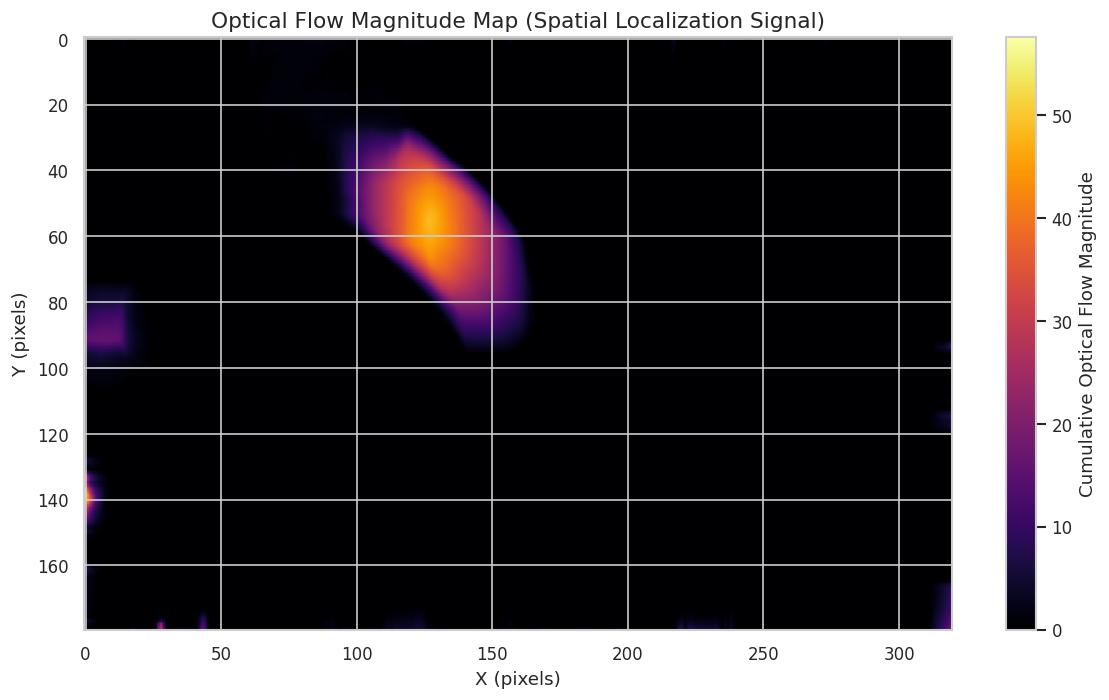
\includegraphics[width=\linewidth]{fig/heatmap.pdf}
    \fbox{\parbox{0.9\linewidth}{\centering\vspace{2em}\textit{[Export motion heatmap from notebook Section 4.2]}\vspace{2em}}}
    \caption{Accumulated flow magnitude on a synthetic calibration video. High values concentrate at the collision site.}
    \label{fig:heatmap}
\end{figure}

\paragraph{Where things go wrong.}
We see three main error patterns. (1) Temporal localization breaks when a camera captures large-scale scene motion, such as wind-blown trees or shifting cloud shadows, that creates frame-difference spikes as large as the collision itself. (2) The spatial centroid drifts toward the center of the frame when background motion is spread evenly across the image, because the weighted average does not isolate a single high-activity cluster. (3) CLIP misclassifies collisions when the surveillance frame resolution is low or the viewpoint is oblique, since CLIP was trained on internet photographs that look quite different from overhead CCTV stills.
